\documentclass{article}

% Language setting
% Replace `english' with e.g. `spanish' to change the document language
\usepackage[english]{babel}

% Set page size and margins
% Replace `letterpaper' with `a4paper' for UK/EU standard size
\usepackage[letterpaper,top=2cm,bottom=2cm,left=3cm,right=3cm,marginparwidth=1.75cm]{geometry}

% Useful packages
\usepackage{amsmath}
\usepackage{graphicx}
\usepackage{commath}
\usepackage{amssymb}
\usepackage{xparse}
\usepackage[colorlinks=true, allcolors=blue]{hyperref}

\NewDocumentCommand{\codeword}{v}{%
\texttt{\textcolor{blue}{#1}}%
}


\title{Project: MIPS MPU}
\author{Pedram Kayedpour}

\begin{document}

\maketitle

\section{Introduction}

The goal of the project is to create a complete Multimedia Processing Unit (MPU) including an Assembler. The MPU design we are going for is a 4 stage piplined processor consisting of stages: Instruction Fetch, Instruction Decode, Execution, and Write Back.

\begin{figure}
	\centering
	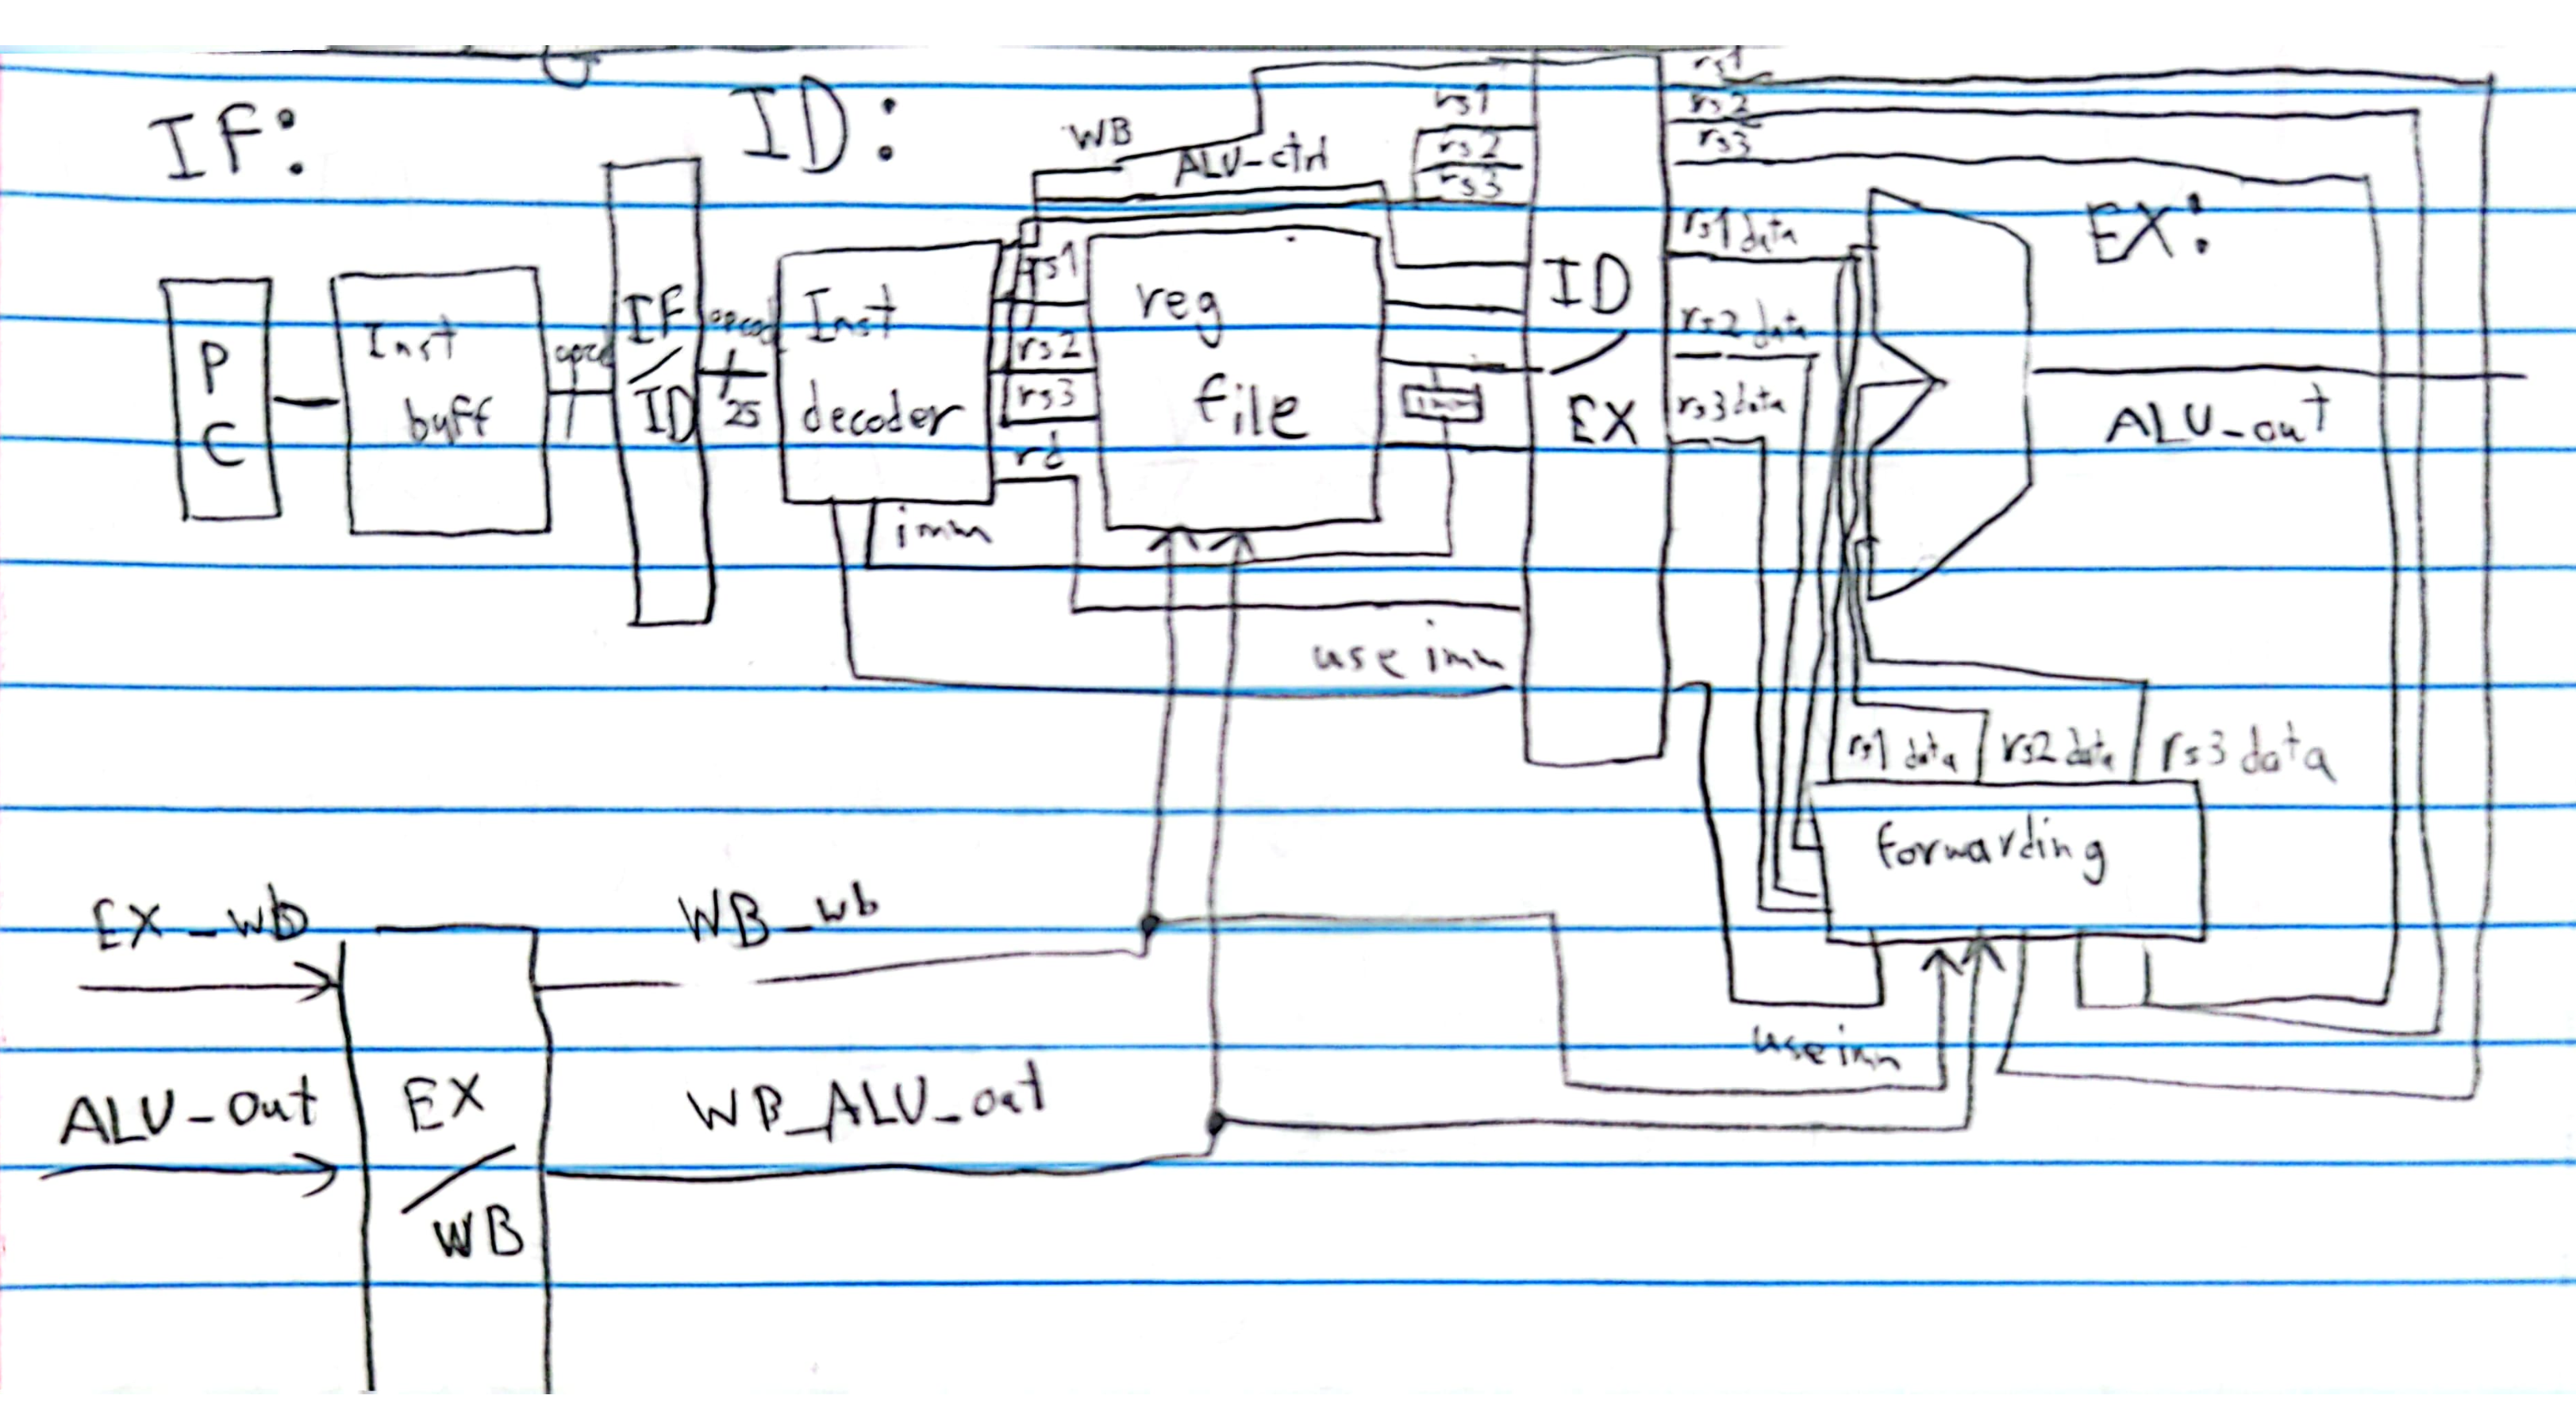
\includegraphics[width=1\linewidth]{diagram.png}
	\caption{Diagram of MPU}
	\label{fig:diagram}
\end{figure}

\section{Design}

The design of the four stage MPU is similar to what we learn in Stony brooks ESE 345 Class. Except there is a main component missing and that is main memory. One more important thing to note when dealing with piplining is that there are hazards that will occur. These hazards in our case our just simply using the same register twice back to back. The solution to this without slowing down is to forward the newest value from the WB stage back to EX stage into the ALU instead of reading from the ID/EX register. Or in other words, Forwarding.

The 0 register is always set to zero as it is with mips architecture.

\subsection{Assembler}

One Important part of any computer architecture is that we needed to make our own Assembler for our mips MPU. The way I decided to approach this was to write an assembler in C. The assembler is pretty good and it is able to handle a pretty soft-typed format. One quirk that it does have, is that BCW needs to have a dummy register filled in or else it wont be able to assemble the mips instruction.

The complier should be able to handle all instruction. This means that this MPU could be tested with as many instructions and combination of instructions as we would like. all that matters is for someone to write the mips instructions and assemble it using the compiler.c file provided with this report.

\section{Testing}

The main method I decided to test the MPU was to feed it a normal and small set of instructions on only the first 2 registers in the register file. My reasoning was that since all registers are the same I would not need to test functionallity of all registers. All I needed to check was wether or not the pipelining was able to handle back to back instructions without having trouble dealing with forwarding or write bypass.

The code given to the MPU is provided in the table below. an image of the waveform is provided in \ref{fig:waveform}.

\section{Results}

\begin{figure}
	\centering
	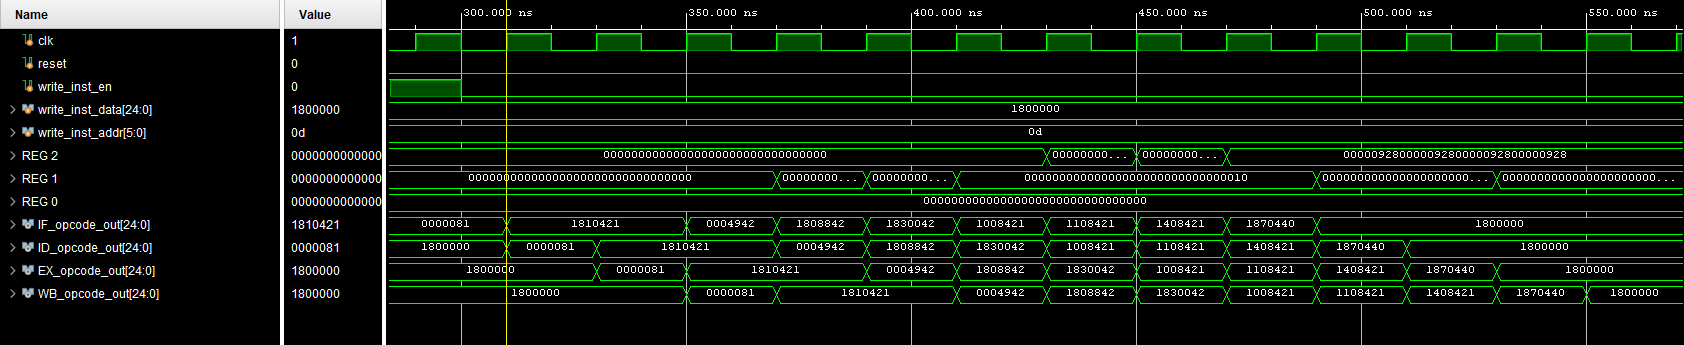
\includegraphics[width=1\linewidth]{imageOP.png}
	\caption{waveform of MPU executing until all OPcodes reach NOP.}
	\label{fig:waveform}
\end{figure}


\begin{center}
	\begin{tabular} {|c||c|c|c|c|}
		\hline
		Cycle & IF & ID & EX & WB \\
		\hline
		\hline
		1 & LI & NOP & NOP & NOP \\
		\hline
		2 & AU & LI & NOP & NOP \\
		\hline
		3 & AU & AU & LI & NOP \\
		\hline
		4 & LI & AU & AU & LI \\
		\hline
		5 & SLHI & LI & AU & AU \\
		\hline
		6 & BCW & SLHI & LI & AU \\
		\hline
		7 & IMAL & BCW & SLHI & LI \\
		\hline
		8 & IMAH & IMAL & BCW & SLHI \\
		\hline
		9 & LMAL & IMAH & IMAL & BCW \\
		\hline
		10 & SFWU & LMAL & IMAH & IMAL \\
		\hline
		11 & NOP & SFWU & LMAL & IMAH \\
		\hline
		12 & NOP & NOP & SFWU & LMAL \\
		\hline
		13 & NOP & NOP & NOP & SFWU \\
		\hline
		14 & NOP & NOP & NOP & NOP \\
		\hline
	\end{tabular}
\end{center}

The expected results of the simulation is that one register (register one) will contain a value that 16 * 16 + 16 and then that number done the same operation of x * x + x. The result for register 2 is that we have a broadcasted word that is in the first 8 hex values. before that reg 2 was shifted to the left twice so it will be the value 586 * 4. Register zero was written to but it should still stay as zero.

\section{Conclusion}

In the final project of Stony Brook University's ESE 345 course, we designed and simulated a 4 stage pipleined mips MPU that is able to do arithmatic on large registers that can contain multiple 16 bit or 32 bit sections. We were able to show the pipelining stages and the flow of instructions through the pipepline.

\end{document}
